
\paragraph{Campo elettrico prodotto da due lastre parallele}

\begin{figure}[h] % plot di un grafico 2D andamento del campo elettrico
\centering
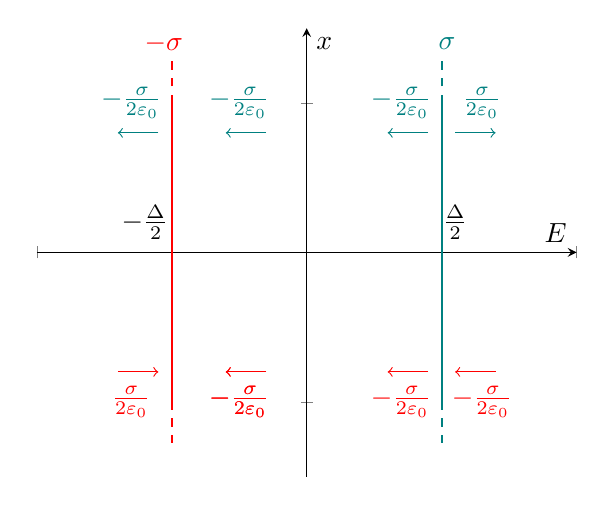
\begin{tikzpicture}
\begin{axis}[
%axis lines = left,
axis x line = center,
axis y line = middle,
xlabel = $E$,
ylabel = $x$,
ymax = 1.5,
ymin = -1.5,
xmax = 2,
xmin = -2,
xtick = {-2,-1,0,1,2},
xticklabels = {, , ,},
ytick = {-2,-1,0,1,2},
yticklabels = { , , , , }
]

\addplot [teal,thick] coordinates {(1,-1) (1,1)};
\addplot [teal,thick,dashed] coordinates {(1,1) (1,1.3)};
\addplot [teal,thick,dashed] coordinates {(1,-1) (1,-1.3)};

\addplot [red,thick] coordinates {(-1,-1) (-1,1)};
\addplot [red,thick,dashed] coordinates {(-1,-1) (-1,-1.3)};
\addplot [red,thick,dashed] coordinates {(-1,1) (-1,1.3)};

\addplot [->,teal] coordinates {(1.1,0.8) (1.4,0.8)};
\addplot [->,teal] coordinates {(0.9,0.8) (0.6,0.8)};
\node [teal] at (axis cs: 1.3,1) {$\frac{\sigma}{2\varepsilon_0}$};
\node [teal] at (axis cs: 0.7,1) {$-\frac{\sigma}{2\varepsilon_0}$};

\addplot [->,teal] coordinates {(-0.3,0.8) (-0.6,0.8)};
\node [teal] at (axis cs: -0.5,1) {$-\frac{\sigma}{2\varepsilon_0}$};

\addplot [->,teal] coordinates {(-1.1,0.8) (-1.4,0.8)};
\node [teal] at (axis cs: -1.3,1) {$-\frac{\sigma}{2\varepsilon_0}$};

\node[] at (axis cs: -1.2,0.2) {$-\frac{\Delta}{2}$};
\node[] at (axis cs: 1.1,0.2) {$\frac{\Delta}{2}$};
\node [teal] at (axis cs: 1.04,1.4) {$\sigma$};
\node [red] at (axis cs: -1.06,1.4) {$-\sigma$};

\addplot [->,red] coordinates {(-1.4,-0.8) (-1.1,-0.8)};
\node [red] at (axis cs: -1.3,-1) {$\frac{\sigma}{2\varepsilon_0}$};

\addplot [->,red] coordinates {(-0.3,-0.8) (-0.6,-0.8)};
\node [red] at (axis cs: -0.5,-1) {$-\frac{\sigma}{2\varepsilon_0}$};

\addplot [->,red] coordinates {(-0.3,-0.8) (-0.6,-0.8)};
\node [red] at (axis cs: -0.5,-1) {$-\frac{\sigma}{2\varepsilon_0}$};

\addplot [->,red] coordinates {(0.9,-0.8) (0.6,-0.8)};
\node [red] at (axis cs: 0.7,-1) {$-\frac{\sigma}{2\varepsilon_0}$};

\addplot [->,red] coordinates {(1.4,-0.8) (1.1,-0.8)};
\node [red] at (axis cs: 1.3,-1) {$-\frac{\sigma}{2\varepsilon_0}$};

\end{axis}
\end{tikzpicture}
\caption{Andamento del campo attraverso due lastre cariche}
\label{fig:lastre_indefinite}
\end{figure}

Siano due lastre poste a distanza $\Delta$ con carica $\sigma$ e $-\sigma$,
si avrà un campo pari a $\frac{\sigma}{2\varepsilon_0}$ a destra della
lastra $\sigma$ e $-\frac{\sigma}{2\varepsilon_0}$ nel lato sinistro della lastra.
Viceversa la lastra sinistra $-\sigma$ avrà verso opposto, applicando la sovrapposizione degli 
effetti si vede che il campo è nullo all'esterno dei due piani e pari a $-\sigma/\varepsilon_0$ 
nel mezzo.
$$
E_z = \begin{cases}
0, & |z| > \frac{\Delta}{2}\\
-\frac{\sigma}{\varepsilon_0}, & |z| \leq \frac{\Delta}{2}
\end{cases}
$$
Questa situazione è analoga a quella presente in un condensatore.

\section{Elettrostatica - Potenziale}
Si riportano le equazioni dell'elettrostatica
$$
\oiint_\Sigma \vec{E}\cdot\hat{n} dS = \frac{Q_{\Omega_\Sigma}}{\varepsilon_0}\ \ \forall\ \Sigma \text{ chiusa}
$$
$$
\oint_\Gamma \vec{E}\cdot\hat{t} dl =0\ \ \forall\ \Gamma \text{ chiusa}
$$
In forma locale diventano
$$
\nabla\cdot\vec{E} = \frac{\rho}{\varepsilon_0} \text{ in } \Omega \text{ punti regolari}
$$
L'equazione di Faraday-Neumann diventa:
$$
\nabla \times \vec{E} = 0 \text{ in } \Omega \text{ punti regolari}
$$
Le condizioni di raccordo si scrivono come:
$$
\begin{aligned}
\hat{n}\cdot (\vec{E}_2 - \vec{E}_1) &= \frac{\sigma}{\varepsilon_0} \text{ su } \partial\Omega\\
\hat{n}\times (\vec{E}_2 - \vec{E}_1) &= 0 \text{ su } \partial\Omega
\end{aligned}
$$

Se il dominio $\Omega$ è a connessione lineare semplice si ottiene l'equazione di \textit{Poisson}
$$
\nabla\times\vec{E} = 0 \Rightarrow \vec{E} = - \nabla V \text{ in } \Omega \Rightarrow \nabla^2V = -\frac{\rho}{\varepsilon_0} \text{ in } \Omega
$$
Sulla frontiera di $\Omega$: 15:06
$$
\hat{n}\cdot\left(-\nabla V_2 + \nabla V_1\right) = \frac{\sigma}{\varepsilon_0} \Leftrightarrow
-\frac{\partial V_2}{\partial n} + \frac{\partial V_1}{\partial n}...
$$


$$
\hat{n}\times\left(\vec{E}_2-\vec{E}_1\right) = 0 \Rightarrow \hat{n}\times\left(-\nabla V_2 + \nabla V_1\right) = 0 \Rightarrow \hat{n}\times\left(-\nabla V_2 + \nabla V_1\right)\cdot\hat{m} = 0
$$
quindi
$$
\hat{t}\cdot\left(\nabla V_2 - \nabla V_1\right) = 0 \Rightarrow \frac{\partial V_2}{\partial n} - \frac{\partial V_1}{\partial n} = 0
$$
$$
\Rightarrow \frac{\partial}{\partial \hat{t}}(V_2-V_1) = 0 \Rightarrow V_2 = V_1
\text{ lungo la direzione }\hat{t}
$$
Si ha quindi continuità del potenziale attraverso le superfici.

Supponiamo che la carica $\rho$ sia nulla in $\Omega$, allora
$$
\nabla^2 V = 0 \in \Omega \text{ equazione di Laplace}
$$
le soluzioni dell'equazione di Laplace sono funzioni armoniche in $\Omega$.

\subparagraph{Proprietà delle funzioni armoniche}

\subparagraph{Proprietà di unicità della soluzione}
$$
\begin{cases}
\nabla^2 V = 0\\
\left.V\right|_{\partial\Omega} = h \in \partial\Omega
\end{cases}
$$
Si dimostra con l'identità di Green
$$
\nabla\cdot(f\nabla f) = f\nabla^2f + (\nabla f)^2
$$
$$
\iiint_\Omega \nabla\cdot(V\nabla V) = ... 34:55
$$

Supponiamo $V_1$ e $V_2$ soluzioni distinte del problema

...

$$
\nabla(\Delta V) = 0 \in \Omega \Rightarrow \Delta V = \text{cost}
$$

Principio del massimo delle funzioni armoniche:
Una funzione armonica in un dominio $\Omega$ assume valori estremi sulla frontiera, se $V$ è costante
su una superficie $\Sigma$, necessariamente deve essere costante nella regione racchiusa $\Omega_\Sigma$.


\subparagraph{Problema di Neumann per l'eq di Laplace}
$$
\begin{cases}
\nabla^2 V = 0 \in \Omega\\
\left.\frac{\partial V}{\partial\hat{n}}\right|_{\partial \Omega} = f \in \partial \Omega
\end{cases}
$$
Dim.
$$
\iiint_{\Omega} \left[\nabla(\Delta V)\right]^2 dV = \iint_{\partial\Omega} \Delta V \frac{\partial\Delta V}{\partial \hat{n}} dS = 0
$$
46:09

\subsection{Calcolo della funzione potenziale in condizioni di simmetria}
\paragraph{Carica puntiforme}
Sia $P_0$ un punto distante $r_0$ dall'origine e $P$ distante $r$ dall'origine.
Si suppone di estendere il raggio $r$ fino alla lunghezza di $r_0$ e di congiungere il punto
ottenuto con $p_0$ mediante una linea che giace sulla circonferenza di pari raggio.

Sia la carica puntiforme localizzata nell'origine, allora
$$
\vec{E}(P) = \frac{Q}{4\pi \varepsilon_0}\frac{1}{r^2} \vec{e}_r
$$
Integrando $\vec{E}$
SCRIVI INTEGRALE 54:54

$$
 = \frac{Q}{4\pi\varepsilon_0}\left(\frac{1}{r} - \frac{1}{r_0}\right)
$$


In genere quando le cariche sono al finito, conviene scegliere come funzione potenziale
$$
V(r) = \frac{Q}{4 \pi \varepsilon_0}\frac{1}{r}
$$

Sia $Q$ una carica nell'origine e $P$ il raggio vettore, il campo è diretto in direzione radiale
mentre le superfici ad $r$ costante hanno tutte lo stesso potenziale.

\subparagraph{Potenziale generato da una distribuzione volumetrica $\rho$}
Sia $\Omega$ una regione carica con densità $\rho(p')$, allora il potenziale elementare sarà
$\rho(p')dV$, di conseguenza
$$
dV = \frac{\rho(p')dV}{4\pi\varepsilon_0}\frac{1}{|\vec{r}_p - \vec{r}_{p'}|} \Rightarrow
\frac{1}{4\pi\varepsilon_0} \iiint_\Omega ... 1:18
$$

$V(p)$ è continua $\forall P \in R^3$

\subparagraph{Potenziale prodotto da distribuzione superficiale $\sigma$}
Sia $S$ la superficie con distribuzione superficiale $\sigma$
$$
dV = \frac{\sigma(p')dS}{4\pi\varepsilon_0} \frac{1}{|\vec{r}_p - \vec{r}_{p'}|} \Rightarrow
\frac{1}{4\pi\varepsilon_0} \iint_S \frac{\sigma(p')}{|\vec{r}_p - \vec{r}_{p'}|} dS = V(p)
$$

\subparagraph{Distribuzione lineare con densità $\lambda(p')$}
1:23

\subparagraph{Operatori differenziali in coordinate curvilinee}
Sia $\Delta\Omega$ un volumetto elementare in $P$ di dimensioni $dl_1,\ dl_2,\ dl_3$.
Siano $(u_1,u_2,u_3)$ un sistema di coordinate curvilinee ortogonali, gli spostamenti elementari
saranno:
\begin{align*}
dl_1 &= h_1du_1\\
dl_2 &= h_2du_2\\
dl_3 &= h_3du_3
\end{align*}
AGGIUNGI SUPERFICI ELEMENTARI

Volume elementare:
$$
dV = dl_1dl_2dl_3 = h_1h_2h_3du_1du_2du_3
$$






\paragraph{Distribuzione di carica superficiale con simmetria sferica}
$$
\frac{1}{r^2}\frac{\partial}{\partial r} \left(r^2 \frac{\partial V}{\partial r}\right) = 0
$$

A B C D costanti di integrazione eccetera AAAAAHAHAHAAA

